%%%%%%%%%%%%%%%%%%%%%%%%%
%% Template for small reports
%%%%%%%%%%%%%%%%%%%%%%%%%

\documentclass[letterpaper,notitlepage,10pt]{article}

%Additional packages
\usepackage{fullpage} %For using small margins 
\usepackage{latexsym}
\usepackage{amssymb}
\usepackage{amsmath}
\usepackage[english]{babel}
\usepackage[pdftex]{color,graphicx} %Images for pdfs
\usepackage[pdftex,colorlinks]{hyperref} %Hyperlinked pdfs
\usepackage{listings} %For adding code
\usepackage{subcaption}

\usepackage{tikz}
\usetikzlibrary{fit,positioning,arrows}

%If you need to add math
\newenvironment{proof}{\begin{trivlist} \item[] {\em Proof:}}{\hfill $\Box$ \end{trivlist}}
\newtheorem{theorem}     {Theorem}
\newtheorem{lemma}       {Lema}
\newtheorem{observation} {Observation}
\newtheorem{proposition} {Proposition}
\newtheorem{conjecture}  {Conjecture}
\newtheorem{corollary}   {Corolari}
\newtheorem{property}    {Property}
\newtheorem{definition}  {Definition}

%Title box
\newcommand{\titlebox}[6]
{\noindent\fbox{\parbox{\textwidth}{#1 \hfill\textbf{#2}\begin{center} 
\LARGE #3 \end{center}#4 $<$\href{mailto:#5}{#5}$>$ \hfill #6}}\bigskip\\}

%If you want to include code
%standard configuration of the listings package
%\lstset{language=matlab, basicstyle=\footnotesize, numbers=left, frame=lines, frameround=tfft,breaklines=true}
%how to include a file "\lstinputlisting{../../Courses/16720-CV/hw2/matlab/blockify.m}"


%%%%%%%%%%%%%%%%%%%%%%
%% Here begins the document
%%%%%%%%%%%%%%%%%%%%%%
\begin{document}
\titlebox
{CMU  - Robotics Institute} % Institution (ex: CMU - Robotics Institute)
{Manipulation Lab}              % Center (ex: Manipulation Lab)
{MLab Simple Hand Documentation}                                  % Title
{Robbie Paolini}             % Author
{rpaolini@cmu.edu}           % e-mail
{2013/07/17}                      % Date (format yyyy/mm/dd)


\section{Introduction}
In this document, we discuss the MLab Simple Hand, and how to control and receive data from it.

\subsection{Hardware Description}

\begin{figure}[h]
\centering
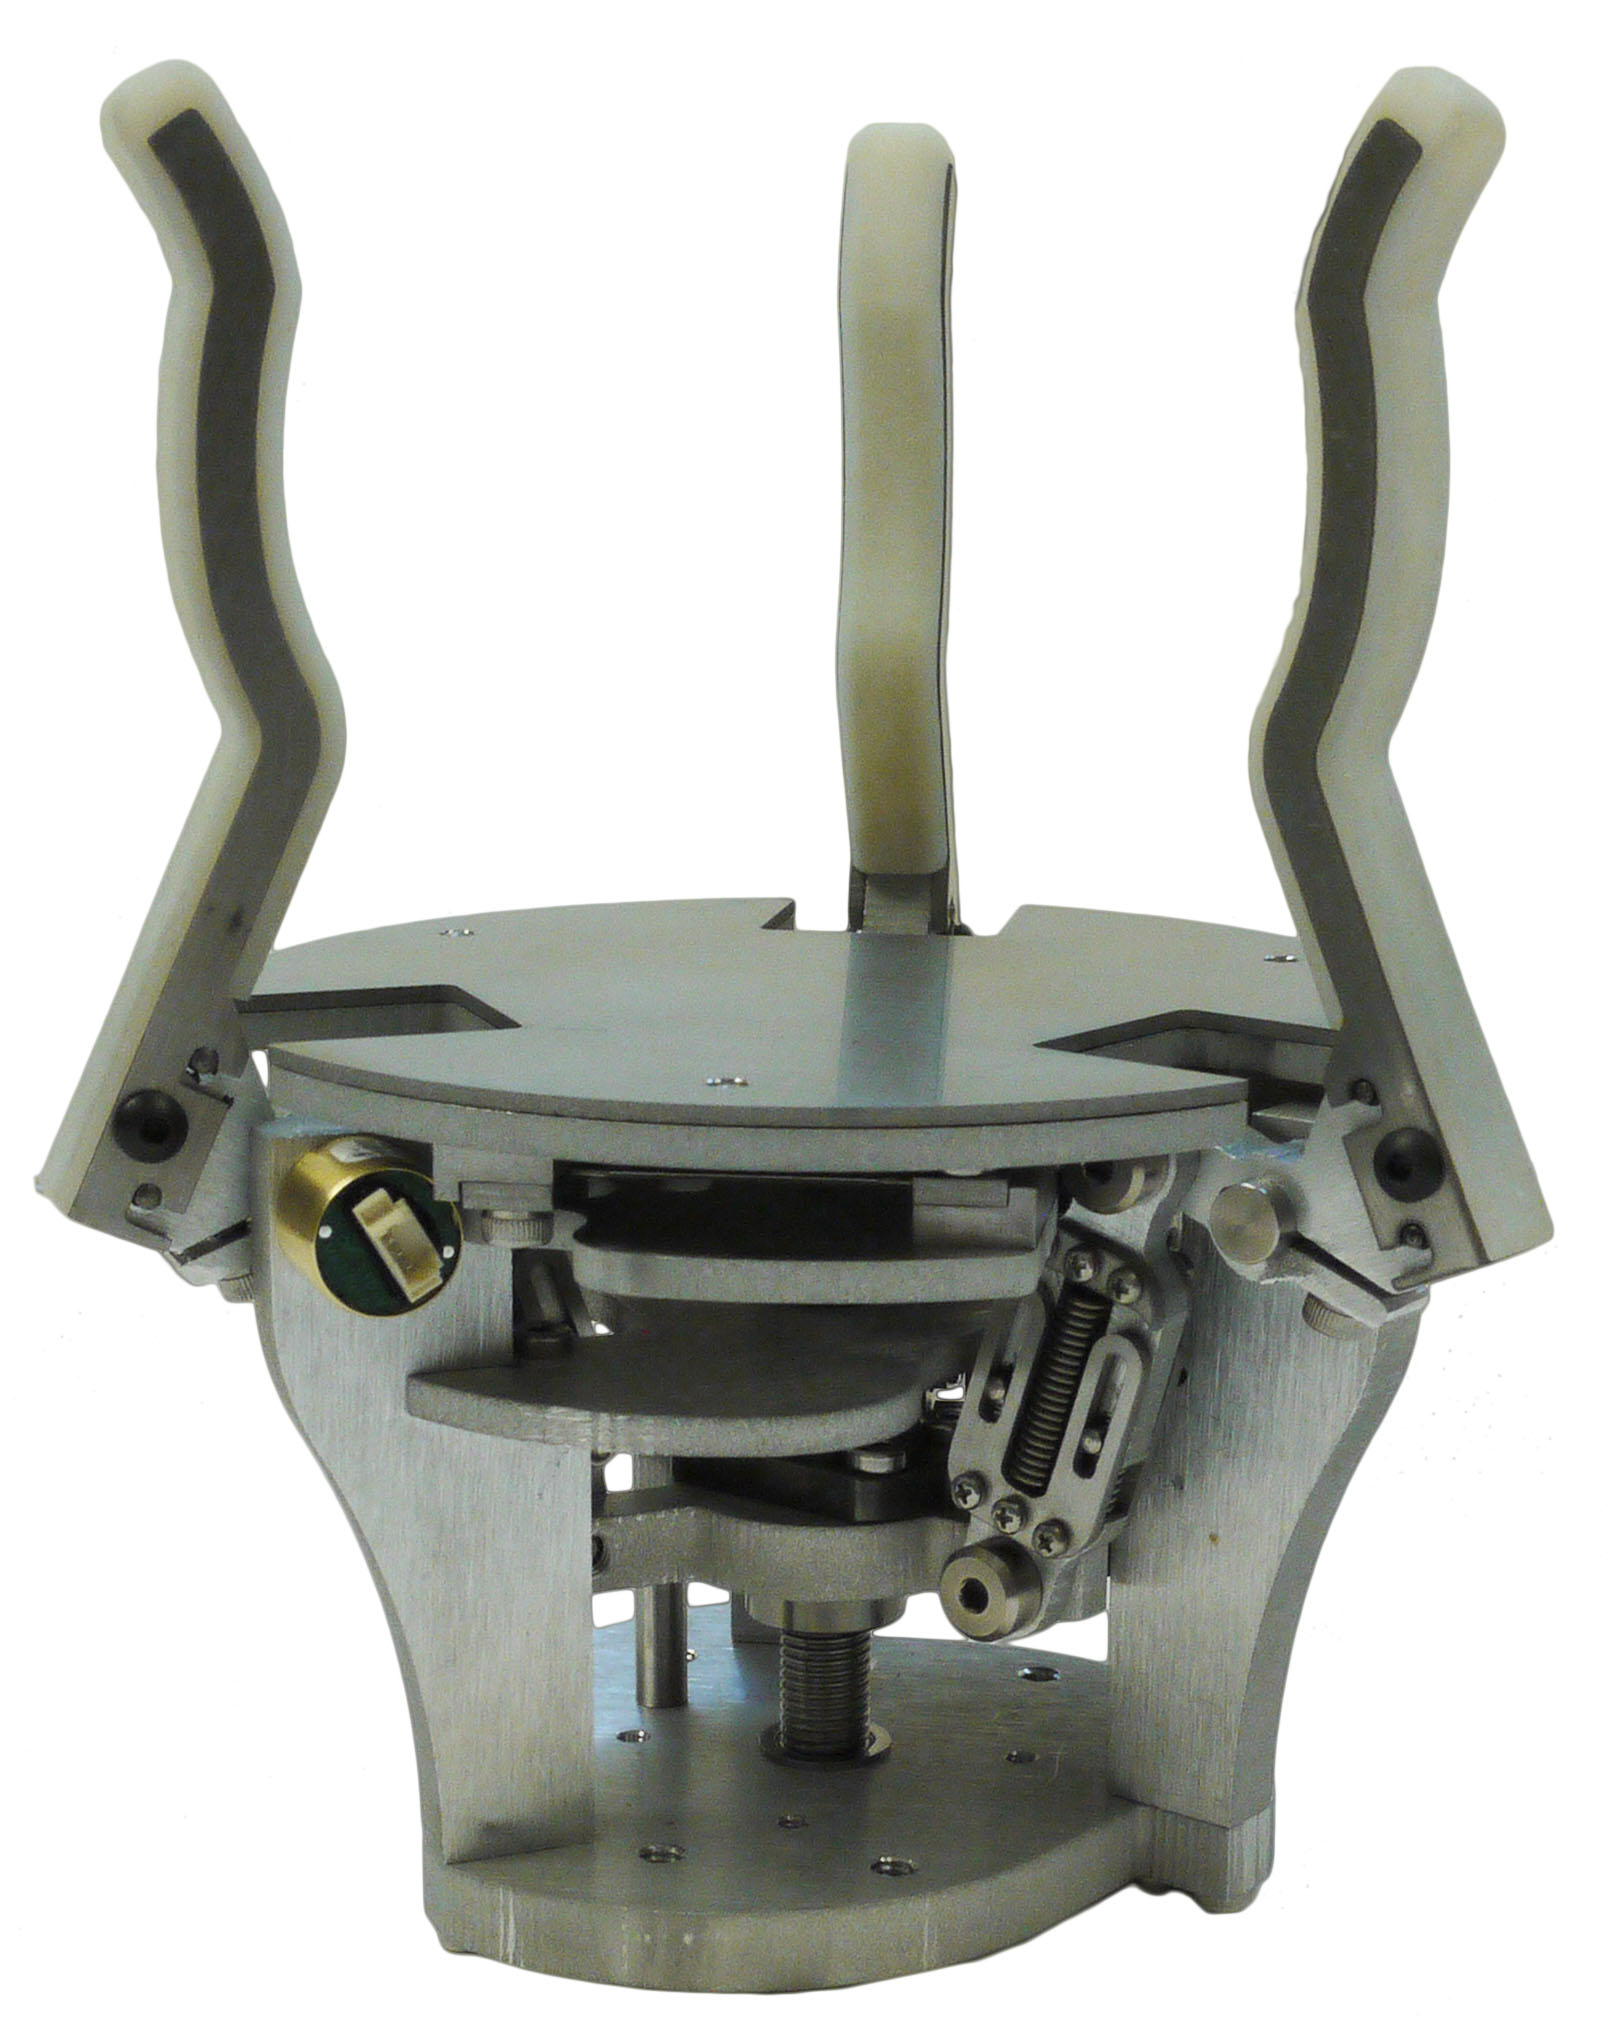
\includegraphics[width=0.25\textwidth]{figures/MLabHand.jpg}
\caption{The MLab Simple Hand}
\label{fig:hand}
\end{figure}

The MLab Simple Hand (Figure~\ref{fig:hand}) has 1 motor for actuation connected to 3 compliantly linked fingers. There is an encoder connected to each of the fingers to get angle information. As each finger is connected to the motor with a spring, given the finger position and motor position, the torque exerted by each finger can also be computed. The hand also has a force sensing palm which allows the user to measure the normal force into the palm and 2 torques around the planar directions on top of the palm. 

The hand is controlled via a USB connection, and must also be connected to a 6V power supply to power the motor. The hand uses an Arduino as its central processor, and thus code can be modified at any time.

\subsection{Angles, Forces, Directions}
Here, we explain the meaning of terms used in the rest of the document.

\begin{itemize}
\item \textbf{Finger Angle:} The angle a finger makes with respect to the hand. As shown in Figure~\ref{fig:hand_diagram}, 0 corresponds to the finger being wide open, $\pi/2$ corresponds to the finger being straight up, and $\pi$ corresponds to the finger being parallel with the palm. Normal values will be around $(\pi/2, \pi)$.
\item \textbf{Motor Angle:} The motor is controlled by encoder counts, but the \emph{motor angle} is the position of the motor for a nominal finger angle. For example, if we specify a motor angle of $2\pi/3$, this will move the motor so that the finger angles will be $2\pi/3$ in the absence of collision or external forces.
\item \textbf{Opening and Closing:} As we increase angle, the fingers close. As we increase the motor encoder count, the hand closes as well. It takes a little over 10000 encoder counts to go from fully open to fully closed.
\item \textbf{Finger torques:} As we push or pull the finger from its nominal location, it exerts a force because of the springs compliantly linking it to the motor. This can be expressed as a torque about the finger rotation axis. We will say that the finger torque is positive if the finger is being pressed open, and negative if the finger is being pulled closed.
\item \textbf{Palm forces and torques:} We can measure planar torques and the normal force using our force sensing palm. As shown in Figure~\ref{fig:hand_diagram}, the $x$-axis corresponds to the vector drawn from the center of the palm out towards the center of the motor (exactly opposite of a finger). The $z$-axis points outwards, and the $y$-axis is specified using the right-hand rule. When we report torques, they will be about the $x$ and $y$ axes, and when we report the normal force, it will be in the $-z$ direction.
\end{itemize}

\begin{figure}[t]
\centering
\begin{subfigure}{0.45\textwidth}
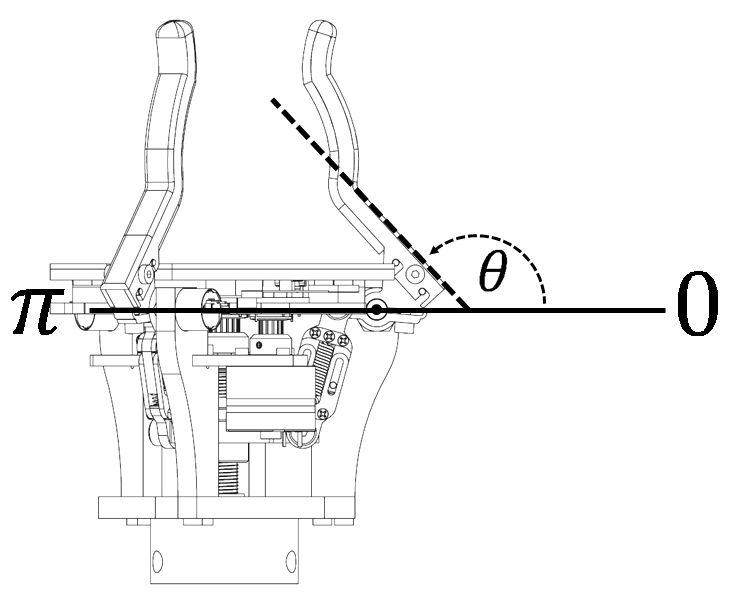
\includegraphics[width=\textwidth]{figures/finger_angle.png}
\end{subfigure}
\quad
\quad
\begin{subfigure}{0.3\textwidth}
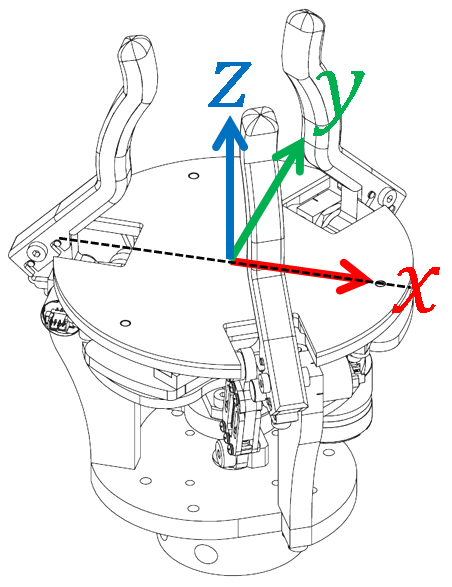
\includegraphics[width=\textwidth]{figures/palm_frame.png}
\end{subfigure}
\caption{Finger angles and palm frame}
\label{fig:hand_diagram}
\end{figure}

\subsection{State Machine}

The hand operates using a very simple state machine, which is shown in Figure~\ref{fig:state_machine}.

\begin{figure}[h]
\centering
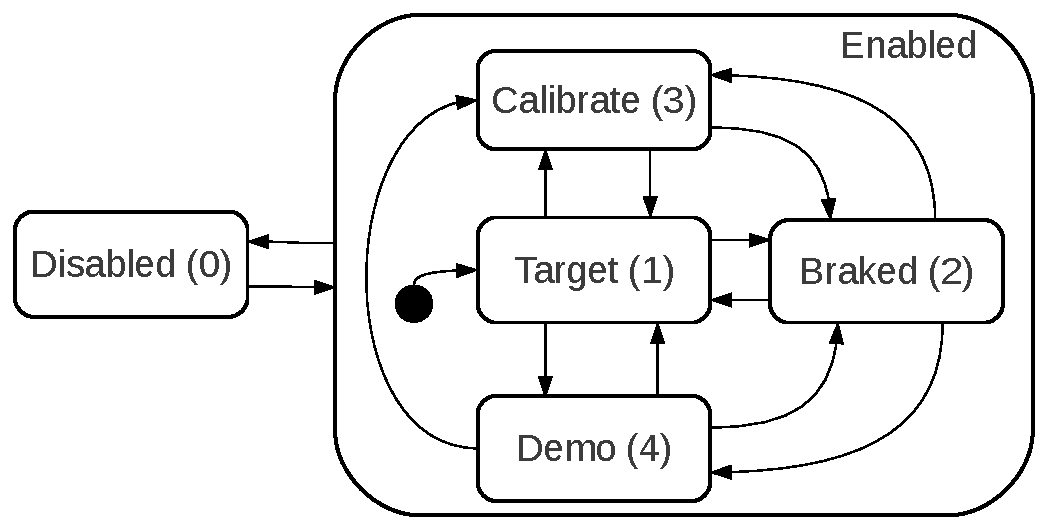
\includegraphics[width=0.8\textwidth]{figures/state_machine.pdf}
\caption{The state machine used by the hand}
\label{fig:state_machine}
\end{figure}

There are 5 states. Disabled (0), Target (1), Braked (2), Calibrate (3), and Demo (4). The numbers in parentheses next to each state is the value that will be returned when the hand is queried for its current state. The table below explains each of the states in more detail: \\

\begin{tabular}{|l|p{0.8\textwidth}|}
\hline
\textbf{State Name} & \textbf{Description} \\ \hline
Disabled & In this state, the motor controlling the hand is disconnected. It can be moved freely by hand. The hand must be enabled before any motion commands can be executed. The hand can be move to the disabled state from any other state. \\ \hline
Target & This is the main motion state. In this state, the hand is servoed to a target position. If the hand is not calibrated, only encoder target commands can be issued. \\ \hline
Braked & In this state, the hand is braked by ``connecting" the leads of the motor together. No power is used and it is harder to turn the motor, but not as strong as when in the Target state. \\ \hline
Calibrate & The hand calibrates itself when in this state. As the motor has an incremental encoder, the encoder is reset by moving the hand to a hard stop. Until the hand is calibrated, finger angles and torques cannot be computed, and no angular motor commands may be issued. \\ \hline
Demo & In this state, we can close and open the hand by pressing on the force sensor. We can only enter this state once the hand has been calibrated. \\ \hline
\end{tabular}

\pagebreak

\section{Control Reference}
The hand is controlled using a serial interface over the USB connection, with a baud rate of 115200. The hand can accept and reply to commands and queries, stream data, and report errors and information.

\subsection{Input}
All commands sent to the hand must look like the following:
\begin{verbatim}
command [arg1] [arg2] ... #
\end{verbatim}


\noindent Below we list possible commands to send to the hand with any necessary arguments:\\

\begin{tabular}{l|p{0.8\textwidth}}
Command & Description \\
\hline
\verb;stop#; & Stops and brakes the motor on the hand. \\
\verb;disable#; & Disables the motor controller. Before any motion commands are sent, an \verb;enable; command must be sent. \\
\verb;enable#; & Enables the motor controller and puts the motor in a \emph{floating} state. \\
\verb;demo#; & Puts hand in demo state. \\
\verb;calibrate#; & Calibrates the motor on the hand. The hand must be calibrated before motion commands are sent. \\
\verb;open#; & Opens the hand as wide as it will go. \\
\verb;open <rad>#; & Opens the hand \verb;<rad>; radians. (rad is a float)\\
\verb;close#; & Closes the hand as much as possible.\\
\verb;close <rad>#; & Closes the hand \verb;<rad>; radians. (rad is a float)\\
\verb;fenc#; & Returns the value of all 3 finger encoders followed by their time stamp. \\
\verb;fenc <n>#; & Returns the value of finger encoder \verb;<n>; and its time stamp. (n is 0, 1, or 2)\\
\verb;fang#; & Returns the current angle in radians of all 3 fingers and their time stamps. \\
\verb;fang <n>#; & Returns the current angle in radians of finger \verb;<n>; and its time stamp. (n is 0, 1, or 2)\\
\verb;ftorque#; & Returns the current torques on the 3 fingers and their time stamps. \\
\verb;ftorque <n>#; & Returns the current torque on finger \verb;<n>; and its time stamp. (n is 0, 1 or 2)\\
\verb;menc#; & Returns the current motor encoder value. \\
\verb;mang#; & Returns the current motor angle. \\
\verb;praw#; & Returns the raw readings from the 3 palm sensors and their time stamps. \\
\verb;praw <n>#; & Returns the raw reading from palm sensor <n> and its time stamp. (n is 0, 1, or 2)\\
\verb;pft#; & Returns the force and torques on the palm. \\
\verb;datadump#; & Returns all information known to the hand at the current time. \\
\verb;mstatus#; & Returns the motion status of the hand. \\
\verb;tune#; & Returns the current motor controller gains. \\
\verb;tune <P> <I> <D>#; &Set the motor controller gains. (P, I, and D are floats)\\
\verb;speed#; & Returns the current speed of the motor. \\
\verb;speed <value>#; & Sets the speed of the motor to \verb;<value>;. (Value is an integer between 0 and 100, representing 0-100\%). \\
\verb;current#; & Returns the current limit of the motor. \\
\verb;current <value>#; & Sets the current limit of the motor to \verb;<value>;. (Value is an integer between 0 and 100, representing 0-100\%). \\
\verb;menc <count>#; & Sets the target and moves the motor to encoder count \verb;<count>;. (count is an integer)\\
\verb;mang <rad>#; & Sets the target and moves the motor to an angle of \verb;<rad>; radians. (rad is a float)\\
\verb;stream#; & Returns the current stream register. \\
\verb;stream <value>#; & Sets up what values to stream. \verb;<value>; is a single character whose 8 bits are a bit array which represent what data to stream. \\


\end{tabular}

\subsection{Streaming Output}
The stream command takes in a single character whose 8 bits are a bit array. Each bit represents a type of data to stream. If it is set to 1, that type of data will be streamed, and if set to 0, it will not. By default, the stream register is initially set to all zeros. We use 8 bits to create our character, with the lowest bit being bit 1, and highest being bit 8:\\

\begin{tabular}{|l|l|}
\hline
bit 1 & Motor Angle \\ \hline
bit 2 & Motor Encoder \\ \hline
bit 3 & Finger Angles \\ \hline
bit 4 & Finger Encoders \\ \hline
bit 5 & Palm Sensors \\ \hline
bit 6 & Palm Forces \\ \hline
bit 7 & Finger Torques \\\hline
bit 8 & Unused \\ \hline
\end{tabular}\\

\noindent Based on the current stream register, different data will be sent over the serial port from the hand. All of the data will be sent back with the following form:
\begin{verbatim}
#X<data>&
\end{verbatim}
where \verb;#; is the start of the mesage, \verb;X; is the data identifier, and \verb;&; is the end of a message. \\

\noindent We list the possible data types and the format of the messages sent back below:\\

\begin{tabular}{l|p{0.8\textwidth}}
Data Format & Description \\
\hline
\verb;#O<ang>&; & Motor angle (radians). \verb;<ang>; is 4 characters long, representing a number with 3 decimal places. (1.234 $\rightarrow$ 1234). \\
\verb;#M<enc>&; & Motor encoder value. \verb;<enc>; is an unsigned integer from 0 to 65536. \\
\verb;#A<a1><a2><a3>&; & Finger angles (radians). \verb;<a*>; are each 4 characters long, representing a number with 3 decimal places (1.234 $\rightarrow$ 1234). \\
\verb;#F<e1><e2><e3>&; & Finger encoder counts. \verb;<e*>; are each 4 characters long, and are integers between 0 and 4095. \\
\verb;#R<s1><s2><s3>&; & Palm sensor readings. \verb;<s*>; are each 4 characters long, and are integers between 0 and 4095. \\
\verb;#P<fz><tx><ty>&; & Palm force and torque. Format of \verb;<fz>, <tx>, <ty>; are tbd. \\
\verb;#T<t1><t2><t3>&; & Finger torques. Format of \verb;<t*>; are tbd. \\

\end{tabular}


\subsection{Response Output}
When a command from the input section is sent to the hand, a response is generated and sent back from the hand. All responses are of the form:
\begin{verbatim}
#QX<message>&
\end{verbatim}
where \verb;#; is the start of the message, \verb;Q; indicates a response, \verb;X; is the message identifier, and \verb;&; is the end of a message. \\

Below we list the different responses generated by the hand after different input messages are sent:\\

\begin{tabular}{l|p{0.6\textwidth}}
Response Format & Description \\
\hline
\verb;#QC<success>&; & Command confirmation. \verb;<success>; will be 0 for a failure to execute the requested action, and 1 if the action was successful. \verb;stop;, \verb;disable;, \verb;enable;, \verb;calibrate;, \verb;open;, \verb;close;, \verb;tune <P> <I> <D>#;, \verb;speed <value>#;, \verb;current <value>#;, \verb;menc <value>#;, \verb;mang <value>#;, and \verb;stream <value>#; will all generate a command confirmation message. \\

\verb;#QM<enc>&; & Motor encoder value. Response generated from a \verb;menc#; message. \verb;<enc>; will be an unsigned integer from 0 to 65535 representing the current motor encoder count. \\

\verb;#QO<ang>&; & Motor angle. Response generated from a \verb;mang#; message. \verb;<ang>; will be a float between 0 at $2\pi$. \\

\verb;#QF<e1>@<t1>,<e2>@<t2>,<e3>@<t3>&; & Finger encoders. Response generated from a \verb;fenc#; message. \verb;<e*>; will be integers from 0 to 4095, and represent the encoder count of the fingers. \verb;<t*>; are the timestamps that these values were measured at, and are unsigned long numbers so will range from 0 to 4294967295. \\

\verb;#QN<en>@<tn>&; & Finger encoder. Response generated from a \verb;fenc <n>#; message. \verb;<en>; and \verb;<tn>; will contain the encoder count and time stamp for finger \verb;<n>; respectively. Encoder count is an integer between 0 and 4095, and time stamp is an unsigned long from 0 to 4294967295. \\

\verb;#QA<a1>@<t1>,<a2>@<t2>,<a3>@<t3>&; & Finger angles. Response generated from a \verb;fang#; message. \verb;<a*>; will be floats from 0 to $2\pi$, and represent the angle of the fingers. \verb;<t*>; are the timestamps that these values were measured at, and are unsigned long numbers so will range from 0 to 4294967295. \\

\verb;#QI<an>@<tn>&; & Finger angle. Response generated from a \verb;fang <n>#; message. \verb;<an>; and \verb;<tn>; will contain the angle and time stamp for finger \verb;<n>; respectively. Angle is a float between 0 and $2\pi$, and time stamp is an unsigned long from 0 to 4294967295. \\

\verb;#QT<v1>@<t1>,<v2>@<t2>,<v3>@<t3>&; & Finger torques. Response generated from a \verb;ftorque#; message. \verb;<v*>; will be floats representing the torque on each of the fingers (units tbd). \verb;<t*>; are the timestamps that these values were measured at, and are unsigned long numbers so will range from 0 to 4294967295. \\

\verb;#QU<vn>@<tn>&; & Finger torque. Response generated from a \verb;ftorque <n>#; message. \verb;<vn>; and \verb;<tn>; will contain the torque and time stamp for finger \verb;<n>; respectively. Torque is a float between with units tbd, and time stamp is an unsigned long from 0 to 4294967295. \\

\verb;#QI<an>@<tn>&; & Finger angle. Response generated from a \verb;fang <n>#; message. \verb;<an>; and \verb;<tn>; will contain the angle and time stamp for finger \verb;<n>; respectively. Angle is a float between 0 and $2\pi$, and time stamp is an unsigned long from 0 to 4294967295. \\

\verb;#QR<s1>@<t1>,<s2>@<t2>,<s3>@<t3>&; & Palm sensors. Response generated from a \verb;praw#; message. \verb;<s*>; will be integers from 0 to 4095, and are each of the palm sensor readings. \verb;<t*>; are the timestamps that these values were measured at, and are unsigned long numbers so will range from 0 to 4294967295. \\

\verb;#QW<sn>@<tn>&; & Palm sensor. Response generated from a \verb;praw <n>#; message.  \verb;<sn>; and \verb;<tn>; will contain the palm sensor reading and time stamp for sensor \verb;<n>; respectively. The sensor reading is an integer between 0 and 4095, and time stamp is an unsigned long from 0 to 4294967295. \\

\end{tabular}

\begin{tabular}{l|p{0.6\textwidth}}
Response Format & Description \\
\hline


\verb;#QP<fz>,<tx>,<ty>&; & Palm forces and torques. Response generated from a \verb;pft#; message. \verb;<fz>; is the normal force, \verb;<tx>; is the torque along the x axis of the palm, and \verb;<ty>; is the torque along the y axis. All values will be floats. units tbd.\\

\verb;#QV<value>&; & Current value. Response generated from a \verb;speed#; or \verb;current#; message. Returns an integer between 0 and 100 representing the current value of the speed or current limit of the hand. \\

\verb;#QG<P>,<I>,<D>&; & Controller Gains. Response generated from a \verb;tune#; message. \verb;<P>;, \verb;<I>;, \verb;<D>; are the current motor controller gains, and are all floats. \\

\verb;#QM<C>&; & Stream register. Response generated from a \verb;stream#; message. \verb;<C>; is a single character which represents the 8-bit array of the stream register to see what the hand is currently streaming. \\

\verb;#QS<C>&; & Motion Status. Response generated from a \verb;mstatus#; message. \verb;<C>; is a single character which represents the 8-bit array of the motion status. See below for an explanation of what each of the bits mean. \\

\end{tabular}

\bigskip

\noindent The motion status bit-array contains information about the status of the hand, from whether or not it is currently moving, to what state it is in, to whether or not it is calibrated. The meaning of the bits are shown below:\\

\begin{tabular}{|l|l|}
\hline
bit 1 & 1 if hand is moving, 0 otherwise \\ \hline
bits 4-2 & Current state we're in. (See state machine explanation.) \\ \hline
bit 5 & 1 if hand is calibrated, 0 otherwise \\ \hline
bits 8-6 & Unused \\ \hline
\end{tabular}

\bigskip

\noindent The only command not covered in our table of responses is the \verb;datadump#; command. This will send a large amount of text over the serial port, and will be sent as an information message, which is covered in the next section.



\subsection{Other Messages}
In addition to the messages mentioned above, there are several more that the hand can send over serial:\\

\begin{tabular}{l|p{0.8\textwidth}}
Message Format & Description \\
\hline
\verb;#E<code>&; & Error message. \verb;<code>; is the integer code of the error received. \\
\verb;#I<message>&; & Information message. \verb;<message>; is a string of variable length that does not contain the \verb;&; character.\\

\end{tabular}

\bigskip

\noindent Different error codes are listed below:\\

\begin{tabular}{|l|l|}
\hline
\textbf{Error Code} & \textbf{Description} \\ \hline
00 & No Error \\ \hline
01 & Unrecognized Command \\ \hline
02 & Hand Not Calibrated Error \\ \hline
03 & Illegal State Change \\ \hline
\end{tabular}\\


%%%%%%%%%%%%%%%%%%%%
%% If you want bibliography
%%%%%%%%%%%%%%%%%%%%
%\bibliographystyle{unsrt}
%\bibliography{} %Name and location of the bibfile

%To cite a reference -> \cite{cite_name}
%To make a reference appear in the bibliography without a citation in the text -> \nocite{cite_name}

\end{document}
